% =====================================================================
%  How the human and two AI agents work together
%  Beamer source, self-contained (no external style file)
%  Compile:  pdflatex human_ai_cowork.tex   (run twice)
% =====================================================================
\documentclass[aspectratio=169,10pt]{beamer}

\usepackage[T1]{fontenc}
\usepackage{amsmath,amssymb}
\usepackage{tikz}
\usepackage{xcolor}
\usetikzlibrary{arrows.meta,positioning,fit,calc,backgrounds}

% --------- palette ----------
\definecolor{ink}     {HTML}{1A1A1A}
\definecolor{inkgray} {HTML}{5A5A5A}
\definecolor{paper}   {HTML}{FBFAF6}
\definecolor{human}   {HTML}{1F4E79}
\definecolor{agent}   {HTML}{2D5F2C}
\definecolor{check}   {HTML}{8B1A1A}
\definecolor{humanbg} {HTML}{DDE6EF}
\definecolor{agentbg} {HTML}{E0EBDC}
\definecolor{checkbg} {HTML}{F7E0DE}

\usefonttheme{serif}
\setbeamercolor{background canvas}{bg=paper}
\setbeamercolor{normal text}{fg=ink}
\setbeamercolor{structure}{fg=ink}
\setbeamercolor{frametitle}{fg=ink,bg=paper}
\setbeamercolor{itemize item}{fg=ink}
\setbeamertemplate{navigation symbols}{}
\setbeamertemplate{itemize item}{\textbullet}
\setbeamertemplate{frametitle}{%
  \vspace{0.30em}%
  \begin{center}%
    {\bfseries\Large\insertframetitle\par}%
    \vspace{0.28em}%
    {\color{ink}\rule{0.86\paperwidth}{0.4pt}}%
  \end{center}%
  \vspace{0.10em}%
}
\setbeamertemplate{footline}{%
  \hbox to \paperwidth{\hfil\itshape\small\insertframenumber\hspace{0.7em}}%
  \vspace{0.35em}%
}

% --------- shared node styles ----------
\tikzset{
  box/.style      ={draw=ink, fill=white, line width=0.6pt,
                    minimum width=2.6cm, minimum height=0.95cm,
                    align=center, font=\small, inner sep=4pt},
  hbox/.style     ={box, draw=human, fill=humanbg, line width=1.0pt,
                    font=\small\bfseries},
  abox/.style     ={box, draw=agent, fill=agentbg, line width=1.0pt,
                    font=\small\bfseries},
  cbox/.style     ={box, draw=check, fill=checkbg, line width=1.0pt,
                    font=\small\bfseries},
  arr/.style      ={-{Stealth[length=2.6mm,width=2mm]}, line width=0.7pt},
  badarr/.style   ={-{Stealth[length=2.6mm,width=2mm]}, line width=0.9pt,
                    color=check},
  note/.style     ={font=\scriptsize\itshape, color=inkgray, align=center},
}
\newcommand{\bottomnote}[1]{%
  \begin{center}{\itshape\small #1}\end{center}}

% =====================================================================
\begin{document}

% ---------------------------------------------------------------- 1
\begin{frame}[plain]
  \vspace{1.5cm}
  \begin{center}
    {\bfseries\Huge Human--AI cowork\par}
    \vspace{0.9cm}
    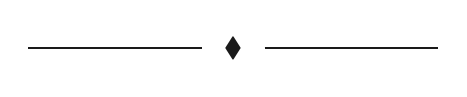
\begin{tikzpicture}
      \draw[ink,line width=0.5pt] (-2.6,0) -- (-0.4,0);
      \node at (0,0) {\color{ink}$\blacklozenge$};
      \draw[ink,line width=0.5pt] (0.4,0) -- (2.6,0);
    \end{tikzpicture}
    \vspace{0.9cm}

    {\Large How one person and two AI agents share one repository\par}
    \vspace{0.5em}
    {\itshape\normalsize\color{inkgray}
      Companion to \texttt{SOP\_HUMAN\_AI\_COWORK.md}\par}
  \end{center}
\end{frame}

% ---------------------------------------------------------------- 2
\begin{frame}{Three parties}
\begin{center}
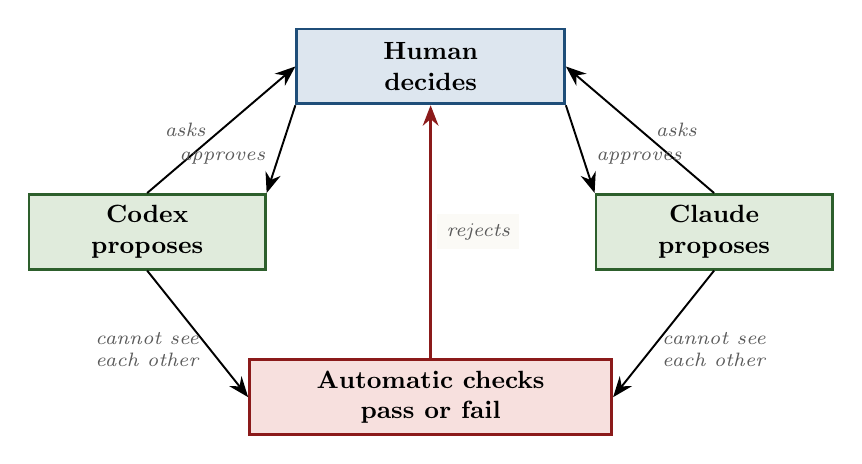
\begin{tikzpicture}[x=1cm,y=1cm]
  \node[hbox,minimum width=3.4cm] (h) at (0,2.1) {Human\\decides};

  \node[abox,minimum width=3.0cm] (c1) at (-3.6,0) {Codex\\proposes};
  \node[abox,minimum width=3.0cm] (c2) at ( 3.6,0) {Claude\\proposes};

  \node[cbox,minimum width=4.6cm] (k) at (0,-2.1)
    {Automatic checks\\pass or fail};

  \draw[arr] (c1.north) -- node[note,left=2pt] {asks} (h.west);
  \draw[arr] (c2.north) -- node[note,right=2pt] {asks} (h.east);
  \draw[arr] (h.south west) -- node[note,left=1pt,pos=0.6] {approves} (c1.north east);
  \draw[arr] (h.south east) -- node[note,right=1pt,pos=0.6] {approves} (c2.north west);
  \draw[arr] (c1.south) -- (k.west);
  \draw[arr] (c2.south) -- (k.east);
  \draw[badarr] (k.north) -- node[note,right=2pt,fill=paper] {rejects} (h.south);

  \node[note,align=left] at (-3.6,-1.5) {cannot see\\each other};
  \node[note,align=left] at ( 3.6,-1.5) {cannot see\\each other};
\end{tikzpicture}
\end{center}
\bottomnote{The two agents never read each other's conversation. Everything one
needs from the other has to be written into the repository.}
\end{frame}

% ---------------------------------------------------------------- 3
\begin{frame}{One shared directory}
\begin{center}
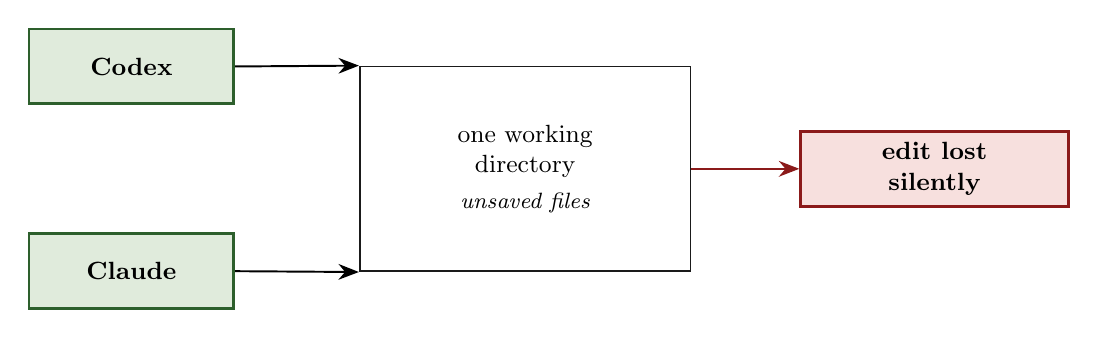
\begin{tikzpicture}[x=1cm,y=1cm]
  \node[abox] (a) at (-4.6, 1.3) {Codex};
  \node[abox] (b) at (-4.6,-1.3) {Claude};
  \node[box,minimum width=4.2cm,minimum height=2.6cm] (d) at (0.4,0)
    {one working\\directory\\[2pt]{\footnotesize\itshape unsaved files}};
  \node[cbox,minimum width=3.4cm] (loss) at (5.6,0) {edit lost\\silently};

  \draw[arr] (a.east) -- (d.north west);
  \draw[arr] (b.east) -- (d.south west);
  \draw[badarr] (d.east) -- (loss.west);
\end{tikzpicture}
\end{center}
\begin{itemize}\setlength{\itemsep}{0.35em}
  \item A branch does not protect an unsaved file
  \item \texttt{git add -A} commits the other agent's work
  \item \texttt{stash}, \texttt{restore}, \texttt{clean} destroy it
\end{itemize}
\bottomnote{Nothing reports the loss, and nothing can recover it.}
\end{frame}

% ---------------------------------------------------------------- 4
\begin{frame}{Separate worktrees}
\begin{center}
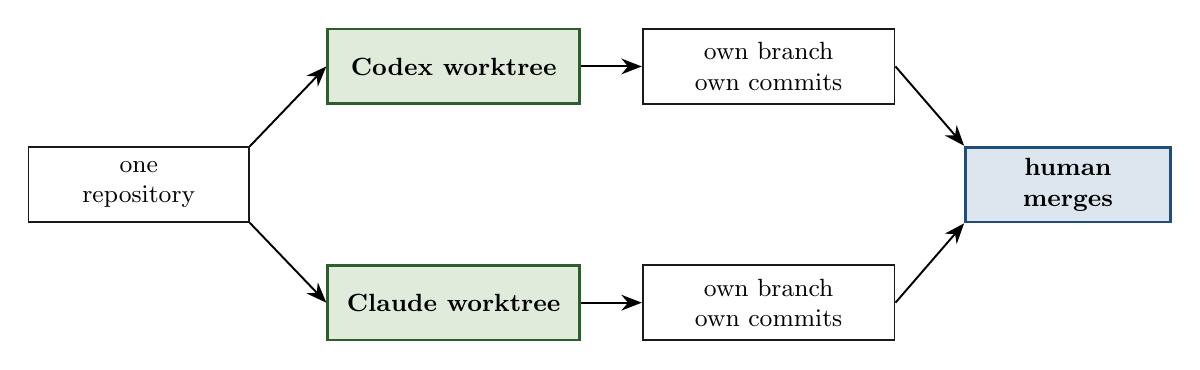
\begin{tikzpicture}[x=1cm,y=1cm]
  \node[box,minimum width=2.8cm] (repo) at (-5.4,0) {one\\repository};

  \node[abox,minimum width=3.2cm] (w1) at (-1.4, 1.5) {Codex worktree};
  \node[abox,minimum width=3.2cm] (w2) at (-1.4,-1.5) {Claude worktree};

  \node[box,minimum width=3.2cm] (b1) at (2.6, 1.5) {own branch\\own commits};
  \node[box,minimum width=3.2cm] (b2) at (2.6,-1.5) {own branch\\own commits};

  \node[hbox,minimum width=2.6cm] (m) at (6.4,0) {human\\merges};

  \draw[arr] (repo.north east) -- (w1.west);
  \draw[arr] (repo.south east) -- (w2.west);
  \draw[arr] (w1.east) -- (b1.west);
  \draw[arr] (w2.east) -- (b2.west);
  \draw[arr] (b1.east) -- (m.north west);
  \draw[arr] (b2.east) -- (m.south west);
\end{tikzpicture}
\end{center}
\bottomnote{The same disagreement still happens. It now arrives as a merge
conflict, which is loud, located, and recoverable, instead of as an edit that
quietly disappeared.}
\end{frame}

% ---------------------------------------------------------------- 5
\begin{frame}{One approval list}
\begin{center}
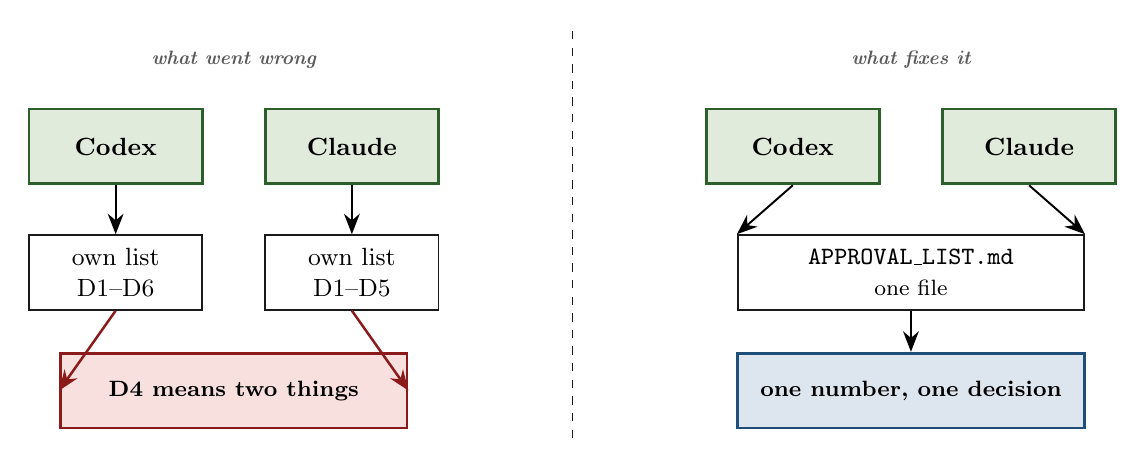
\begin{tikzpicture}[x=1cm,y=1cm]
  % the failure
  \begin{scope}[shift={(-4.3,0)}]
    \node[note] at (0,2.1) {\bfseries what went wrong};
    \node[abox,minimum width=2.2cm] (x1) at (-1.5,1.0) {Codex};
    \node[abox,minimum width=2.2cm] (x2) at ( 1.5,1.0) {Claude};
    \node[box,minimum width=2.2cm] (l1) at (-1.5,-0.6) {own list\\D1--D6};
    \node[box,minimum width=2.2cm] (l2) at ( 1.5,-0.6) {own list\\D1--D5};
    \draw[arr] (x1) -- (l1);
    \draw[arr] (x2) -- (l2);
    \node[cbox,minimum width=4.4cm] (bad) at (0,-2.1)
      {\footnotesize D4 means two things};
    \draw[badarr] (l1.south) -- (bad.west);
    \draw[badarr] (l2.south) -- (bad.east);
  \end{scope}
  % the fix
  \begin{scope}[shift={(4.3,0)}]
    \node[note] at (0,2.1) {\bfseries what fixes it};
    \node[abox,minimum width=2.2cm] (y1) at (-1.5,1.0) {Codex};
    \node[abox,minimum width=2.2cm] (y2) at ( 1.5,1.0) {Claude};
    \node[box,minimum width=4.4cm] (l3) at (0,-0.6)
      {\texttt{APPROVAL\_LIST.md}\\{\footnotesize one file}};
    \draw[arr] (y1.south) -- (l3.north west);
    \draw[arr] (y2.south) -- (l3.north east);
    \node[hbox,minimum width=4.4cm] (ok) at (0,-2.1)
      {\footnotesize one number, one decision};
    \draw[arr] (l3) -- (ok);
  \end{scope}
  \draw[ink,dashed,line width=0.5pt] (0,-2.7) -- (0,2.5);
\end{tikzpicture}
\end{center}
\bottomnote{Read the file, take the number it says is next, and write the proposal
into it in the same message that asks. This is the one step that stays
synchronous.}
\end{frame}

% ---------------------------------------------------------------- 6
\begin{frame}{Naming a thing}
\begin{center}
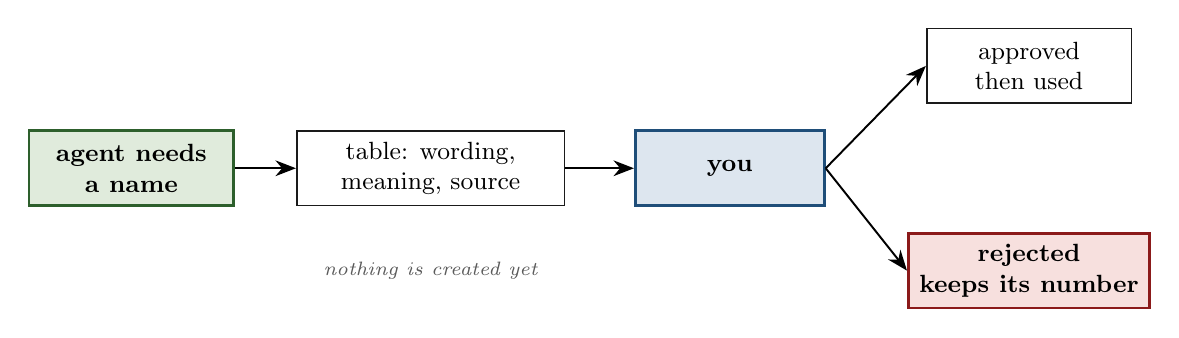
\begin{tikzpicture}[x=1cm,y=1cm]
  \node[abox,minimum width=2.6cm] (need) at (-6.2,0) {agent needs\\a name};
  \node[box,minimum width=3.4cm] (tab) at (-2.4,0)
    {table: wording,\\meaning, source};
  \node[hbox,minimum width=2.4cm] (you) at (1.4,0) {you};
  \node[box,minimum width=2.6cm] (yes) at (5.2, 1.3) {approved\\then used};
  \node[cbox,minimum width=2.6cm] (no) at (5.2,-1.3) {rejected\\keeps its number};

  \draw[arr] (need) -- (tab);
  \draw[arr] (tab) -- (you);
  \draw[arr] (you.east) -- (yes.west);
  \draw[arr] (you.east) -- (no.west);
  \node[note] at (-2.4,-1.3) {nothing is created yet};
\end{tikzpicture}
\end{center}
\begin{itemize}\setlength{\itemsep}{0.35em}
  \item Names a reader sees need approval first
  \item Loop variables and temporaries do not
  \item Silence is not approval
\end{itemize}
\bottomnote{A term passes only if someone new understands it without a glossary.
If it needs the explanation, it is replaced by the explanation.}
\end{frame}

% ---------------------------------------------------------------- 7
\begin{frame}{Commits between agents}
\begin{center}
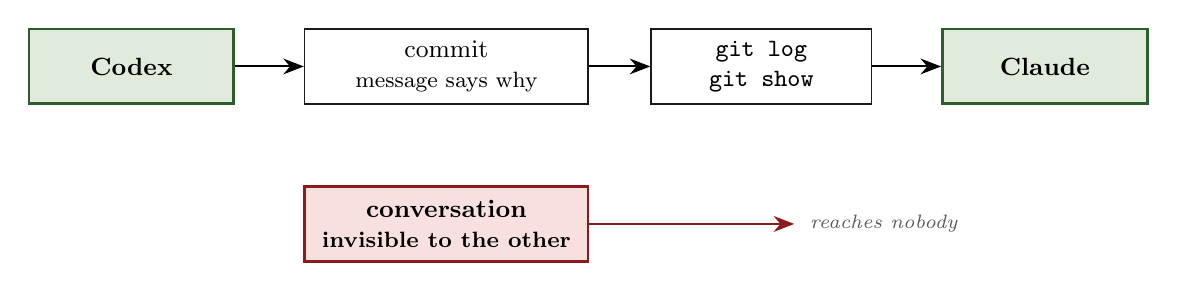
\begin{tikzpicture}[x=1cm,y=1cm]
  \node[abox,minimum width=2.6cm] (a) at (-5.6,0) {Codex};
  \node[box,minimum width=3.6cm] (com) at (-1.6,0)
    {commit\\{\footnotesize message says why}};
  \node[box,minimum width=2.8cm] (log) at (2.4,0) {\texttt{git log}\\\texttt{git show}};
  \node[abox,minimum width=2.6cm] (b) at (6.0,0) {Claude};

  \draw[arr] (a) -- (com);
  \draw[arr] (com) -- (log);
  \draw[arr] (log) -- (b);

  \node[cbox,minimum width=3.6cm] (chat) at (-1.6,-2.0)
    {conversation\\{\footnotesize invisible to the other}};
  \draw[badarr] (chat.east) -- ++(2.6,0) node[note,right=2pt] {reaches nobody};
\end{tikzpicture}
\end{center}
\begin{itemize}\setlength{\itemsep}{0.35em}
  \item One subject per commit
  \item The message says why, not only what
  \item Stage explicit paths, never everything
\end{itemize}
\bottomnote{No separate record is kept, because Git history already is one.}
\end{frame}

% ---------------------------------------------------------------- 8
\begin{frame}{Who decides}
\begin{center}
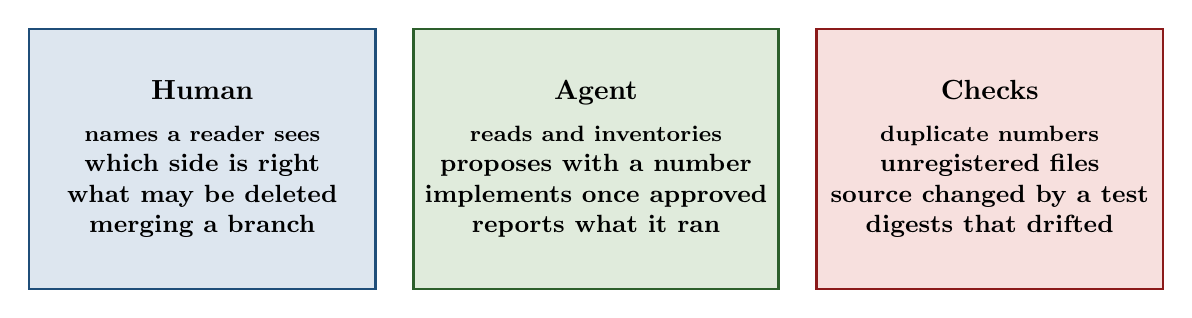
\begin{tikzpicture}[x=1cm,y=1cm,font=\footnotesize]
  \node[hbox,minimum width=4.4cm,minimum height=3.3cm,align=center] (h) at (-5.0,0)
    {\normalsize Human\\[4pt]
     \footnotesize names a reader sees\\
     which side is right\\
     what may be deleted\\
     merging a branch};
  \node[abox,minimum width=4.4cm,minimum height=3.3cm,align=center] (a) at (0,0)
    {\normalsize Agent\\[4pt]
     \footnotesize reads and inventories\\
     proposes with a number\\
     implements once approved\\
     reports what it ran};
  \node[cbox,minimum width=4.4cm,minimum height=3.3cm,align=center] (c) at (5.0,0)
    {\normalsize Checks\\[4pt]
     \footnotesize duplicate numbers\\
     unregistered files\\
     source changed by a test\\
     digests that drifted};
\end{tikzpicture}
\end{center}
\bottomnote{An agent that must ask about everything is useless, and one that may
decide anything is unsafe. Both lists are kept short on purpose.}
\end{frame}

% ---------------------------------------------------------------- 9
\begin{frame}{Checks bind}
\begin{center}
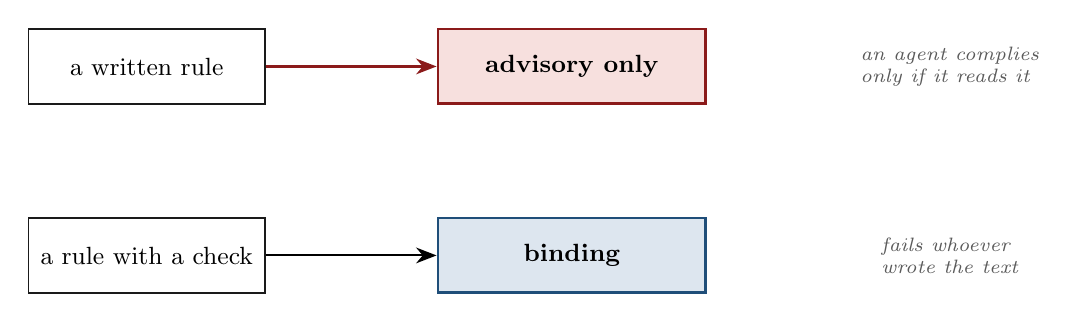
\begin{tikzpicture}[x=1cm,y=1cm]
  \node[box,minimum width=3.0cm] (rule) at (-4.8,1.2) {a written rule};
  \node[cbox,minimum width=3.4cm] (adv) at (0.6,1.2) {advisory only};
  \node[note,align=left] at (5.4,1.2) {an agent complies\\only if it reads it};

  \node[box,minimum width=3.0cm] (rule2) at (-4.8,-1.2) {a rule with a check};
  \node[hbox,minimum width=3.4cm] (bind) at (0.6,-1.2) {binding};
  \node[note,align=left] at (5.4,-1.2) {fails whoever\\wrote the text};

  \draw[badarr] (rule) -- (adv);
  \draw[arr] (rule2) -- (bind);
\end{tikzpicture}
\end{center}
\begin{itemize}\setlength{\itemsep}{0.35em}
  \item An agent here ran Git against a prohibition
  \item The style checker gave seventeen false reports
  \item A check that cries wolf is soon ignored
\end{itemize}
\bottomnote{Fixing the check is part of the work, and the fix is reported.}
\end{frame}

% ---------------------------------------------------------------- 10
\begin{frame}{Takeaway}
\vfill
\begin{center}
  
\begin{tikzpicture}
    \node[draw=ink,fill=white,line width=0.7pt,
          minimum width=13.6cm,minimum height=2.2cm,
          align=center,inner sep=8pt]
      {\bfseries\large One desk each, one list of decisions,\\[3pt]
       \bfseries\large one history both agents can read.\\[8pt]
       \normalsize\itshape The human decides. The checks bind.};
  \end{tikzpicture}
\end{center}
\vfill
\end{frame}

\end{document}
